% !TEX root = document.tex

\chapter{Designing Codex}
\label{chap:designing-codex}

In the previous chapter,~\cref{chap:code-exploration-services},
we concluded that there exists a problem analogous to the IDE portability problem with existing systems that provide code exploration services.
All such existing systems are narrow in scope.
We called this problem the \problem{\times} problem for code exploration services.
In this chapter we will design a prototype system we call the Codex that aims to solve this problem by being less narrow in scope.

Note that Codex is the name of the entire prototype we design, as well as the name for the metadata format used by the prototype.
We will always refer to the \emph{Codex metadata format} explicitly when we refer to the format rather than the prototype in its entirety.

In order for Codex to be less narrow in scope than existing solutions,
Codex will have to support both multiple code exploration media, as well as multiple programming languages.
To do this while avoiding the \problem{\times} problem for code exploration services, Codex needs to consist of two kinds of components:
language-specific systems that can provide information about a program written in a specific language,
and language agnostic systems that can create code exploration services from this information.
Any pair of such systems should be able to work together, to make the complexity \problem{+}.
We will call the language-specific systems Codex metadata generators, or metadata generators for short,
and we call the language-agnostic systems presentation generators.

\section{Code Exploration in Static Media}\label{sec:code-exploration-in-static-media}

Comparing this to \ac{LSP}, metadata generators are analogous to language servers, with presentation generators taking the role of editors.
Note that we were careful to say that presentation generators take the role of an editor, presentations themselves do not.
Although we explore code through some kind of presentation of the code in a medium, together with editor services,
many media have important restrictions on what we can do in them.

Take PDF documents as an example.
While an editor can dynamically make requests to a language server running in the background to get up-to-date information about the program which is written,
we cannot make requests like that inside a PDF document.
We illustrate this in figure \cref{fig:static-vs-dynamic}.

Instead, if we want to provide code exploration services in a PDF document, those need to be embedded into the PDF itself at the moment the PDF is generated.
This baking-in process may involve colouring some text in the document, notably the parts where source code is presented,
and, for example, adding extra hyperlinks to navigate between different pieces of source code.
This embedding is done by the presentation generator, making \emph{it} analogous to an editor with the capability to access language-specific metadata.
In that way, the presentation generated by the presentation generator has the possibility to be entirely static.

\begin{figure}
    \centering
    \begin{tikzpicture}[font={\xkcd}]

        \begin{pgflowlevelscope}{\pgftransformscale{3}}
            \draw (0.75,1.333) node {\faUser};
        \end{pgflowlevelscope}

        \draw[-stealth, ultra thick, draw={rgb:red,128;green,29;blue,39}](3,4) -- (4,4);
        \draw (3.5,4.5) node {Uses};

        \node [draw, thick, shape=rectangle, minimum width=2cm, minimum height=2cm, anchor=center] at (5,4) {};
        \draw (5,4.25) node {PDF};
        \draw (5,3.75) node {Document};

        \draw (7.5,5.5) node {Can't};
        \draw (7.5,5) node {make};
        \draw (7.5,4.5) node {requests};
        \draw[-stealth, ultra thick, draw={rgb:red,128;green,29;blue,39}](6,4) -- (9,4);

        \begin{pgflowlevelscope}{\pgftransformscale{2}}
            \draw (3.75, 2) node {\faTimes};
        \end{pgflowlevelscope}

        %%%%%%%%%%%%%%%%%%%%%%%%%%%

        \begin{pgflowlevelscope}{\pgftransformscale{3}}
            \draw (0.75,2.666) node {\faUser};
        \end{pgflowlevelscope}

        \draw (3.5,8.5) node {Uses};
        \draw[-stealth, ultra thick, draw={rgb:red,128;green,29;blue,39}](3,8) -- (4,8);

        \node[draw, thick, shape=rectangle, minimum width=2cm, minimum height=2cm, anchor=center] at (5,8) {};
        \draw (5,8) node {Editor};

        \draw[-stealth, ultra thick, draw={rgb:red,128;green,29;blue,39}](6,8) -- (9,8);
        \draw (7.5,9) node {Requests};
        \draw (7.5,8.5) node {from};

        \node[draw, thick, shape=rectangle, minimum width=2cm, minimum height=2cm, anchor=center] at (10,8) {};
        \draw (10,8.25) node {Language};
        \draw (10,7.75) node {Server};


        %%%%%%%%%%%%%%%%%%%%%%%%%%%
        \begin{pgflowlevelscope}{\pgftransformscale{3}}
            \draw (0.75,0) node {\faUser};
        \end{pgflowlevelscope}

        \draw[-stealth, ultra thick, draw={rgb:red,128;green,29;blue,39}](3,0) -- (4,0);
        \draw (3.5,0.5) node {Uses};

        \node [draw, thick, shape=rectangle, minimum width=2cm, minimum height=2cm, anchor=center] at (5,0) {};
        \draw (5,0.25) node {PDF};
        \draw (5,-0.25) node {Document};

        \draw (7.5,1) node {Generates};
        \draw (7.5,0.5) node {PDF};
        \draw[stealth-, ultra thick, draw={rgb:red,128;green,29;blue,39}](6,0) -- (9,0);

        \node[draw, thick, shape=rectangle, minimum width=2cm, minimum height=2cm, anchor=center] at (10,0) {};
        \draw (10,0.5) node {Language};
        \draw (10,0) node {Agnostic};
        \draw (10,-0.5) node {Tool};

        \draw (12.5,1.0) node {Generates};
        \draw (12.5,0.5) node {Metadata};
        \draw[stealth-, ultra thick, draw={rgb:red,128;green,29;blue,39}](11,0) -- (14,0);

        \node[draw, thick, shape=rectangle, minimum width=2cm, minimum height=2cm, anchor=center] at (15,0) {};
        \draw (15,0.5) node {Language};
        \draw (15,0) node {Specific};
        \draw (15,-0.5) node {Tool};

    \end{tikzpicture}

    \caption{
        Although a language-agnostic editor can directly make requests to a language-specific source of information (as is the case with \ac{LSP}),
        this architecture cannot work in code exploration media where making requests are impossible such as in PDF documents.
        Code Exploration Services must instead be embedded in such media whenever they are generated.
    }
    \label{fig:static-vs-dynamic}
\end{figure}

\section{Making Metadata Language-Agnostic}\label{sec:making-metadata-language-agnostic}

Between metadata generators and presentation generators, information needs to be exchanged to enable code exploration services.
This information is metadata, information \emph{about} a program which is analysed.
For example, this metadata may be information about which parts of a program references which other parts of a program to facilitate code navigation.

It is important that the way this metadata is stored is in no way tied to any specific programming language.
If that were the case, we are unnecessarily limiting the scope of Codex, just like the narrow tools we discussed in~\cref{sec:code-exploration-services-in-other-media}.
Despite the success of \ac{LSP}, \ac{LSP} too made this mistake.
In \ac{LSP}, a symbol can fall into one of a limited set of categories, which is the symbol's \texttt{SymbolKind}~\autocite{lsp_symbol_kind}.

It is not difficult to find languages with symbol kinds that do not fit into these limited number of categories: Rust has structs but a struct is not a valid \texttt{SymbolKind}, and Haskell's typeclasses fail to fit in as well.
Although substitutes could be used, a struct might become a class, and a typeclass an interface, this does not always work.
C++ has both classes and structs, should these both be labelled as classes in \ac{LSP}?

The approach \ac{LSP} takes, with a limited number of categories into which all languages must fit is doomed to fail.
Because of the wide variety of programming languages in existence, and subtle differences in meaning of language constructs between languages,
we cannot make an exhaustive list of syntactical categories which applies to every language there is.

\subsection{Hierarchical Categorisation}\label{subsec:hierarchical-categorisation}

An approach that avoids making such an exhaustive list was first used for TextMate, an editor for MacOS~\autocite{textmate}.
This approach is now used in facilitating syntax highlighters in multiple editors, also Visual Studio Code.

TextMate uses custom syntax specifications of languages in the form of regular-expression based grammars in order to support syntax colouring.
Such grammars would give different syntactical elements a label.
Colour themes could then apply different colours to items with different labels.
Because the people who make grammars were not necessarily the same as the people making the themes,
a standardised labelling system had to be invented such that all themes could be compatible with all grammars.

Instead of making an exhaustive list, TextMate uses a hierarchical approach, which is not so different from taxonomies in biology.
In TextMate, an \texttt{=} in a variable assignment in Rust might be labelled \texttt{keyword.operator.assignment.rust}.
The dots in this label separate parts of the label, going from generic to specific.
First of all, the \texttt{=} is a keyword, but more specifically an operator, specifically meant for assignment, specifically in Rust.

Now, TextMate themes can match on these labels in a similar way to how CSS classes match:
if a theme only knows how to colour keywords, this assignment operator gets the same colour as all keywords.
However, a theme can also specify a specific colour for all \texttt{keyword.operator}s, or even more specific.
The advantage is that this system can both capture all the language-specific details of syntax,
as well as being easy to read for tools which might not be aware of these language-specific details.

In the Codex metadata format, to be completely language-agnostic,
it makes sense to make any language-specific labelling such as syntactical categories hierarchical.

\section{Generating All Metadata At The Same Time}\label{sec:generating-all-metadata-at-the-same-time}

\ac{LSP} is usually Lazy.
Only when an editor needs information for editor services, it makes a request to the Language Server for it.
In contrast, presentation generators generate a presentation of all the source code at the same time,
embedding code exploration services into the medium.
This process needs access to \emph{all} metadata at the same time.

Thus, a request-response model like \ac{LSP} makes little design for communication between metadata generators and presentation generators.
Instead, a more instantaneous method of communication can be used: a data format instead of a protocol.
This has several advantages.


%vendor lock-in
%some langs can't get static analysis

